\documentclass{standalone}
\usepackage{tikz}
\usetikzlibrary{shapes, backgrounds}
\begin{document}
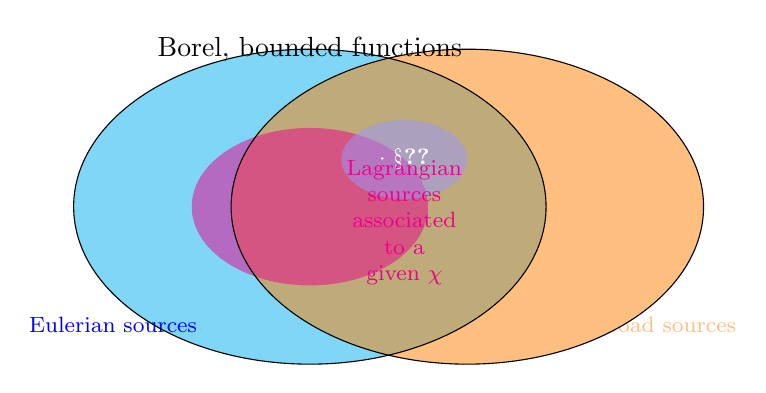
\begin{tikzpicture}
    \def\firstcircle{(0,0) ellipse (3 and 2)}
    \def\secondcircle{(0:2cm) ellipse (3 and 2)}
    
    \begin{scope}[fill opacity=0.5]
        \fill[color=cyan] \firstcircle;
        \fill[color=orange] \secondcircle;
        \fill[color=magenta] (0,0) ellipse (1.5 and 1);
        \fill[color=blue!40] (1.2,0.6) ellipse (0.8 and 0.5);
    \end{scope}
    
    \begin{scope}[every node/.style={font=\footnotesize, inner sep=0.5pt}]
        \node at (-2.5,-1.5) (A) {\textcolor{blue}{Eulerian sources}};
        \node at (4.5,-1.5) (B) {\textcolor{orange!50}{Broad sources}};
        \node at (1.2,0.6) (C) {\textcolor{white}{$\cdot$ \S \ref{sub:nonlocal_formulation_in_current_configuration}}};
        \node[text width=1.5cm, align=center] at (1.2,-0.2) (D) {\textcolor{magenta}{Lagrangian sources\\ associated to a given $\chi$}};
    \end{scope}
    
    \draw \firstcircle node[below left=10pt] {};
    \draw \secondcircle node[below right=10pt] {};
    \node at (0,2) {Borel, bounded functions};
\end{tikzpicture}
\end{document}